\def\pReal{\ensuremath{\operatorname{\mathfrak{Re}}(z)}} % Parte real
\def\pIm{\ensuremath{\operatorname{\mathfrak{Im}}(z)}} % Parte imaginaria

\begin{enunciado}{\ejercicio}
Graficar en el plano complejo
\begin{enumerate}[label=\roman*)]
 \item $\{z \en \complejos / \pReal + 5\pIm \leq 8\}$
 \item $\{z \en \complejos - \{0\} / |z| \geq 2 \text{ y } \frac{\pi}{4} \leq \arg(z) \leq \frac{2\pi}{3}\}$
 \item $\{z \en \complejos - \{0\} / \pIm > 2 \text{ y } \arg(-i \cdot z) = \frac{\pi}{4}\}$
 \item $\{z \en \complejos - \{0\} / \arg(z^4) = \arg((-1 + i)\cdot \bar{z}^2)\}$
\end{enumerate}
\end{enunciado}

\usetikzlibrary{calc}

% ---- 1er grupo -----
%1er grafico
\begin{minipage}{0.44\textwidth}
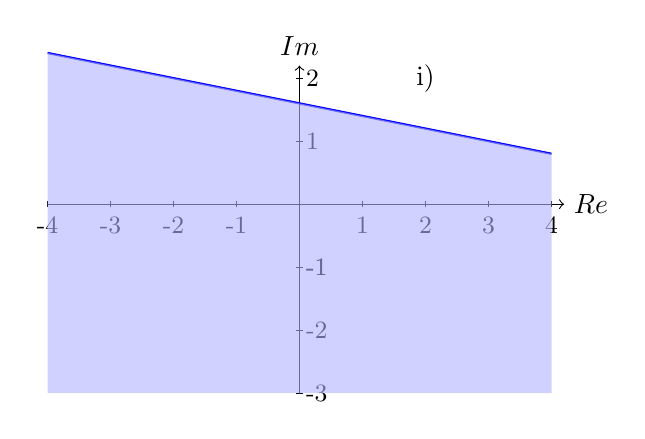
\begin{tikzpicture}[scale=0.8]

%Ejes
\draw[->] (-4, 0) -- (4.2, 0) node[right] {$\mathfrak{Re}$};
\draw[->] (0, -3) -- (0, 2.2) node[above] {$\mathfrak{Im}$};

\foreach \x in {-4, -3, -2, -1, 1, 2, 3, 4} {
\draw (\x, 0.05) -- (\x, -0.05) node[below] {\small \x};
    }

\foreach \y in {-3, -2, -1, -1, 1, 2} {
\draw (0.05, \y) -- (-0.05, \y) node[right] {\small \y};
    }

%Grafico
\draw[thick, blue] (-4, 2.4) -- (4, 0.8) node[right] {};
\fill[blue!30, opacity=0.6]
(-4, 2.4) -- (-4, -3) -- (4, -3) -- (4, 0.8) -- cycle; 

%Name
\node at (2, 2) {i)};

\end{tikzpicture}
\end{minipage}
%2do grafico
\hfill
\begin{minipage}{0.44\textwidth}
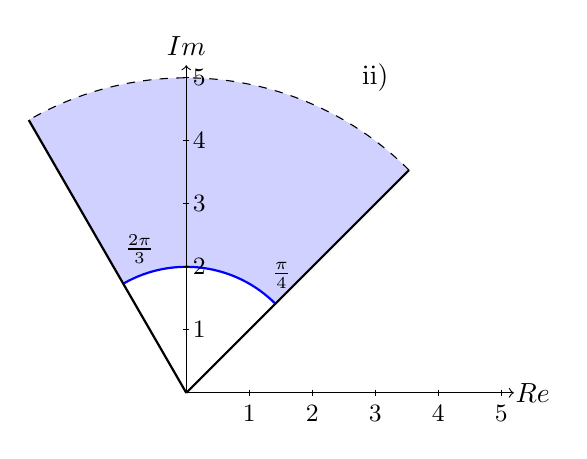
\begin{tikzpicture}[scale=0.8]

%Angulos
\def\startAngle{45}   % pi/4
\def\endAngle{120}    % 2pi/3
\def\innerRadius{2}
\def\outerRadius{5}

% Fill 
\fill[blue!30, opacity=0.6]
    (\startAngle:\innerRadius)
    arc[start angle=\startAngle, end angle=\endAngle, radius=\innerRadius] --
    (\endAngle:\outerRadius)
    arc[start angle=\endAngle, end angle=\startAngle, radius=\outerRadius] --
    cycle;

% Circular Arcs
\draw[thick, color=blue] (45:2) arc[start angle=\startAngle, end angle=\endAngle, radius=\innerRadius];
\draw[dashed] (45:5) arc[start angle=\startAngle, end angle=\endAngle, radius=\outerRadius];

%Ejes
\draw[->] (0,0) -- (5.2,0);
\draw[->] (0,0) -- (0,5.2);
\foreach \x in {1, 2, 3, 4, 5} {
\draw (\x, 0.05) -- (\x, -0.05) node[below] {\small \x};
    }

\foreach \y in {1, 2, 3, 4, 5} {
\draw (0.05, \y) -- (-0.05, \y) node[right] {\small \y};
    }

% Radial lines
\draw[thick] (0,0) -- (\startAngle:\outerRadius);
\draw[thick] (0,0) -- (\endAngle:\outerRadius);

% Labels
\node at (51:\innerRadius + 0.4) {\small $\frac{\pi}{4}$};
\node at (108:\innerRadius + 0.4) {\small $\frac{2\pi}{3}$};
\node at (5.5, 0) {$\mathfrak{Re}$};
\node at (0, 5.5) {$\mathfrak{Im}$};

%Name
\node at (3, 5) {ii)};

\end{tikzpicture}
\end{minipage}

% ---- 2do grupo ---- 
%3er grafico
\begin{minipage}{0.44\textwidth}
\begin{tikzpicture}[scale=0.8]

  % Axes
  \draw[->] (-4, 0) -- (4.2, 0) node[right] {$\mathfrak{Re}$};
  \draw[->] (0, -1) -- (0, 5.2) node[above] {$\mathfrak{Im}$};
  \foreach \x in {-4, -3, -2, -1, 1, 2, 3, 4} {
    \draw (\x, 0.05) -- (\x, -0.05) node[below] {\small \x};
    }

    \foreach \y in {-1, 1, 2, 3, 4, 5} {
    \draw (0.05, \y) -- (-0.05, \y) node[right] {\small \y};
    }
  
  % Horizontal line y = 2
  \draw[dashed, gray] (-4, 2) -- (4, 2);
  \node[right, gray] at (4, 2) {\small $\operatorname{\mathfrak{Im}}(z) = 2$};

  % Grafico
  \draw[thick, blue, ->] (-2, 2) -- (-4, 4) node[above left] {};
  \draw[dashed, blue] (0, 0) -- (-2, 2) node[above left] {};
  \draw[->, blue] (0:0.3) arc[start angle=0, end angle=135, radius =0.3] node[above right, xshift = 3.25, yshift = -0.4] {$\frac{3\pi}{4}$};

  %Name
  \node at (3, 4) {iii)};

\end{tikzpicture}
\end{minipage}
\hfill
%4to grafico
\begin{minipage}{0.44\textwidth}
\begin{tikzpicture}[scale=0.8]

  %Ejes
  \draw[->] (-4, 0) -- (4.2, 0) node[right] {$\mathfrak{Re}$};
  \draw[->] (0, -1) -- (0, 5.2) node[above] {$\mathfrak{Im}$};
  \foreach \x in {-4, -3, -2, -1, 1, 2, 3, 4} {
    \draw (\x, 0.05) -- (\x, -0.05) node[below] {\small \x};
    }

    \foreach \y in {-1, 1, 2, 3, 4, 5} {
    \draw (0.05, \y) -- (-0.05, \y) node[right] {\small \y};
    }

  % Grafico
  \draw[thick, blue] (0, 0) -- (4, 1.6568) node[above left] {};
  \draw[->, blue] (0:1.7) arc[start angle=0, end angle=22.5, radius =1.7] node[below right, yshift=2.75, xshift=1.5] {$\frac{\pi}{8}$};

  %Name
  \node at (3, 4) {iv)};


\end{tikzpicture}
\end{minipage}

Ahora la explicacion de cada región. Pero antes vamos a dejar escritas unas identidades que vamos a tener que usar:
\begin{center}
$\arg(zw) = \arg(z) + \arg(w) - \red{2k\pi}$, $\arg(z^n) = n\cdot \arg(z) - \red{2k\pi}$, $\arg(\bar{z}) = \arg(z) - \red{2k\pi} \quad k \en \enteros$

Los terminos en rojo simplemente son offsets y es para asegurar que el angulo quede entre $0$ y $2\pi$. Las demostraciones de los primeros dos se pueden encontar
en el apunte de Teresa en el apartado $6.3.2$ y $6.3.3$, y el ultimo se puede probar combinando $6.3.2$ y $6.3.1$ (tambien hay otras maneras, no es la unica)
\end{center}

\begin{enumerate}[label=\roman*)]
 \item Podemos tratar a la parte real como el eje x y la imaginaria como el eje y, luego haciendo despejes nos queda
 $y \leq \frac{8 - x}{5}$ que esta descrito por la region dibujada. 
 \item Tenemos que el modulo de $z$ es mayor o igual a 2, asique va a ser la parte externa de la circunferencia 
 de radio 2, luego hay restricciones en el angulo (argumento), descritas en el dibujo. 
 \item Acá hay que operar un poco, ya sabemos que la región si o si va a estar por arriba de 2 en la parte imaginaria, pero 
 el angulo no esta descrito explicitamente, usando las identidades de arriba tenemos $\arg(-i\cdot z) = \arg(-i) + \arg(z) = \frac{\pi}{4}
 \sii \frac{6\pi}{4} + \arg(z) = \frac{\pi}{4} \sii \arg(z) = \frac{-5\pi}{4} = \frac{3\pi}{4}$
 \item Vemos que la unica restriccion es el angulo, operamos y lo encontramos: $\arg(z^4) = \arg((-1 + i)\cdot \bar{z}^2)
 \sii 4\arg(z) = \arg(-1 + i) + \arg(\bar{z}^2) \sii 4\arg(z) = \frac{3\pi}{4} - 2\arg(z) \sii \arg(z) = \frac{3\pi}{24} = \frac{\pi}{8}$
\end{enumerate}

\begin{aportes}
 \item \aporte{https://github.com/sigfripro}{sigfripro \github}
\end{aportes}